
%(BEGIN_QUESTION)
% Copyright 2010, Tony R. Kuphaldt, released under the Creative Commons Attribution License (v 1.0)
% This means you may do almost anything with this work of mine, so long as you give me proper credit

Sketch connecting wires to allow this data acquisition unit (DAQ) to sense strain using quarter-bridge strain gauge circuits on input channels \#2 and \#3, such that increasing tension on the strain gauge (increasing gauge resistance) generates a more {\it positive} signal voltage on each channel:

$$\includegraphics[width=15.5cm]{i04586x01.eps}$$

\underbar{file i04586}
%(END_QUESTION)





%(BEGIN_ANSWER)

\noindent
{\bf Partial answer:}

\vskip 10pt

Note that this is not the only valid solution:

$$\includegraphics[width=15.5cm]{i04586x02.eps}$$

%(END_ANSWER)





%(BEGIN_NOTES)

$$\includegraphics[width=15.5cm]{i04586x03.eps}$$

\vskip 20pt \vbox{\hrule \hbox{\strut \vrule{} {\bf Suggestions for Socratic discussion} \vrule} \hrule}

\begin{itemize}
\item{} Once students show complete, valid sketches for connecting both bridges to the DAQ inputs, challenge them to re-draw the circuits in different configurations which will also work.
\end{itemize}

%INDEX% Pictorial circuit review (analog signal wiring to data acquisition unit)

%(END_NOTES)

